% 导言区
\documentclass[UTF8]{article}%book ,report ,letter


\usepackage{diagbox}
\usepackage{ctexcap}%采用中文标题宏包(标题是中文的)
\usepackage{graphicx}%图片包
\usepackage{color}%彩色文本
\usepackage{amsmath}
\usepackage{hyperref} %超链接包
%覆盖超链接红框
\hypersetup{
	colorlinks=true,
	linkcolor=black
}

\title{\heiti 统计学习方法笔记}
\author{\kaishu 李晨辉}
\date{\today}

% 正文区(文稿区)
\begin{document}
	\maketitle %让头部内容在正文区显示
	\tableofcontents
	\flushleft
	\section{概论}
	泛化误差上界:至少以$1-\delta$的概率有$R(F)<=\hat{R}(f)+\epsilon(d,N,\delta)$
	\section{感知机}
	\begin{enumerate}
		\item 感知机是一种线性分类模型,属于判别模型
		\item 模型:寻找分离超平面;
		\item 损失函数:误分类样本到超平面的距离,误分类样本数不适用因为不连续;
		\item 学习算法:随机梯度下降
	\end{enumerate}
	
	\section{K近邻}
	三要素:
	\begin{enumerate}		
		\item[1.]k值的选择
		\item[2.] 距离度量
		\item[3.] 分类决策规则
	\end{enumerate}
	\subsection{kd树}
	kd树是一种二叉树,表示对k维空间的一个划分;
	通常,依次选择坐标轴对空间进行切分,选择训练实例点在选定坐标轴的中位数为切分点,这样得到的kd树是平衡的。(平衡的kd树的搜索效率未必是最高的)
	
	\section{朴素贝叶斯}
		\begin{enumerate}
			\item 生成模型,学习联合概率分布
			\item 基本假设:用于分类的特征在类确定的条件下是条件独立的(特征向量$X$的每一维度对于输出的条件独立性)
			\item 后验概率最大化等价于期望风险最小化,推导:
			\begin{itemize}
				\item 假设采用0-1损失函数,朴素贝叶斯法的期望风险是对于联合分布$P(X,Y)$取的,因此相当于对于给定输出类别时的条件期望求和$$R_{exp}(f)=E_X\sum\limits_{k=1}^K[L(c_k,f(X))]P(c_k|X)$$
				\item 则对于给定的输入$x$,使其后验概率最大化的类别即为使期望风险最小化的输出。
			\end{itemize}
		\item 损失函数:误分类样本到超平面的距离,误分类样本数不适用因为不连续;
		\item 学习算法:随机梯度下降
		\item 贝叶斯估计
		
	\end{enumerate}

	\section{决策树}
	学习步骤:特征选择、决策树的生成、决策树的修剪
	\subsection{基本概念}
		\begin{enumerate}
			\item 熵(entropy):表示随机变量不确定性的度量$P(X=x_i)=p_i, i=1,2,...,n$,则其熵为:$$H(X)=-\sum\limits_{i=1}^n p_i\log p_i$$
			可以看出,熵的取值只与$X$的分布有关而与其取值无关,因此也可以记为:$$H(p)=-\sum\limits_{i=1}^n p_i\log p_i$$
			\item 条件熵:设有随机变量$(X,Y)$的联合概率分布为:$$P(X=x_i,Y=y_j)=p_{ij}, i=1,2,...,n, j=1,2,...,m$$
			在给定$X$的条件下$Y$的条件熵记为:$H(Y|X)$,定义为$X$给定条件下$Y$的条件概率分布的熵对$X$的数学期望:
			$$H(Y|X)=\sum\limits_{i=1}^n p_iH(Y|X=x_i)$$
			一般的,$$H(X,Y)=-\sum\limits_{x\in X} \sum\limits_{y \in Y } p(x,y)\log p(x,y)$$
			$$H(Y|X)=H(X,Y)-H(X) $$
			\item 信息增益:表示得知特征$X$的信息而使得类别$Y$的信息的不确定性较少的程度;一般地,
			$H(Y)-H(Y|X)$成为$(X,Y)$的互信息,	而特征$A$对训练数据集$D$的信息增益$g(D,A)$为:$$g(D,A)=H(D)-H(D|A)$$
			\item 信息增益比:特征$A$对训练数据集$D$的信息增益比$g_R(D,A)$定义为:
			$$g_R(D,A)=\frac{g(D,A)}{H_A(D)}$$
			$${H_A(D)}=-\sum_{i=1}^{n}\frac{|D_i|}{|D|}\log_2\frac{|D_i|}{|D|}$$
		\end{enumerate}

	\subsection{决策树的生成}
	\subsubsection{ID3算法}
	思想:从根节点,在每一个节点上选择当前信息增益最大的特征作为结点特征,由该特征的不同取值建立子节点,再对子节点递归运用上述算法,直到所有特征的信息增益很小或没有特征可以选择为止,得到一棵决策树。\\
	\emph{注意事项: }在子节点上进行的是特征对训练数据的子集计算信息增益。
	\subsubsection{C4.5算法}
	对ID3算法进行了改进,在生成过程中用信息增益比来选择特征。
	\subsection{决策树剪枝}
	决策树的损失函数定义为:
	$$C_\alpha(T)=C(T)+\alpha|T|
				 =-\sum_{t=1}^{|T|}\sum_{k=1}^{K}N_{tk}\log\frac{N_{tk}}{N_t}$$
	$C(T)$表示模型对训练数据的预测误差,$|T|$表示模型的复杂度(树的深度),$\alpha\geq0$平衡二者之间的关系。
	\\进行剪枝时,将某一组的叶节点回缩至其父节点,若收缩后新的损失不大于旧的损失,则进行剪枝(收缩)。
	\subsection{CART算法}
	\subsubsection{最小二乘回归树}
	\newpage
	\subsubsection{CART决策树}
	利用基尼指数作为决策指标,对所有可能的特征及其所有可能的取值计算在对应处切分,计算基尼指数,选择基尼指数最小的切分点将训练集划分为两个子集,在子集上递归调用上述方法,直到满足停止条件。
	\subsubsection{CART剪枝}
	对整体树$T_0$中的每一个节点$t$,计算$$g(t)=\frac{C(t)-C(T_t)}{|T_t|-1}$$
	其中,$C(t)$是以$t$为单结点树的训练误差,$C(T_t)$是以$t$为根节点的子树$T_t$的训练误差,$|T_t|$是子树$T_t$的叶节点数。
	\\从$T_0$中减去$g(t)$最小的子树$T_t$,将得到的子树记为$T_1$,再从$T_1$减去$g(t)$最小的子树,如此循环下去直到决策树变为只剩根节点。
	\\最后采用交叉验证法从$T_0,T_1,...,T_n$中选出最优子树$T_\alpha$
	
	\section{逻辑斯蒂回归与最大熵模型}
	\subsection{逻辑斯蒂回归模型}
	对于二项LR模型,它的形式是
	$$P(Y=1|x)=\frac{\exp(w \cdot x+b)}{1+\exp(w \cdot x+b)}$$
	$$P(Y=0|x)=\frac{1}{1+\exp(w \cdot x+b)}$$
	把两个式子统一得到似然函数,然后取对数,对于对数似然函数求极大值得到w的估计值即可。
	对于过拟合问题可以采用L1正则化或者L2正则化。
	\subsection{最大熵模型}
	最大熵模型通俗点讲可以理解在满足约束条件的模型中选取熵最大的,对于给定的输入模型的输出是条件概率$P(Y|X)$;\\
	对条件熵的最大化过程可以转化为其负值得最小化,然后引入拉格朗日乘子将约束优化问题转化为它的无约束优化问题,
	然后再对它的对偶问题进行求解,将极小极大问题转化为极大极小问题,先求出最优的满足约束条件的最大熵模型,再对模型进行参数优化。
	\newpage
	\section{支持向量机}
	间隔最大化的直观解释:对训练数据以充分大的确信度进行分类。\\
	SMO:序列最小化(sequential minimal optimization)
	
	\newpage
	\section{集成学习Adaboost}
	\begin{figure}[h]%%图
		\centering  %插入的图片居中表示
		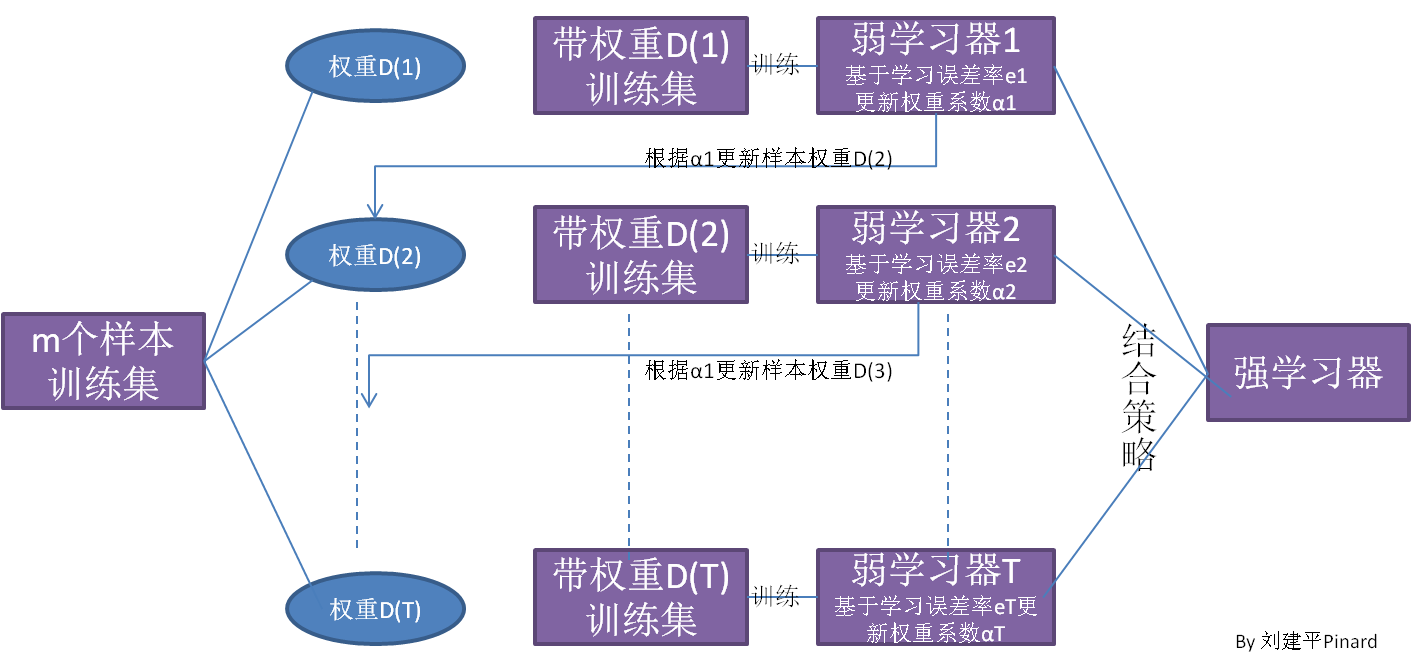
\includegraphics[width=1.0\linewidth]{figures/adaboost}  %插入的图,包括JPG,PNG,PDF,EPS等,放在源文件目录下
		\caption{boosting算法基本思想}  %图片的名称
		\label{boosting}   %标签,用作引用
	\end{figure}
	\subsection{ Adaboost的分类问题}
	训练集的在第k个弱学习器的输出权重为:$$D(k) = (w_{k1}, w_{k2}, ...w_{km}) ;\;\; w_{1i}=\frac{1}{m};\;\; i =1,2...m$$ $m$为样本个数,$i$对应第$i$个样本,初始权重$ w_{1i}$不失一般性的取均值$ w_{1i}=\frac{1}{m}$\\
	对于二分类问题,第k个弱分类器$Gk(x)$在训练集上的加权误差率为:
	$$e_k = P(G_k(x_i) \neq y_i) = \sum\limits_{i=1}^{m}w_{ki}I(G_k(x_i) \neq y_i)$$
	第k个弱分类器$G_k(x)$的权重系数为:$$\alpha_k = \frac{1}{2}log\frac{1-e_k}{e_k}$$
	权重系数更新公式:$$w_{k+1,i} = \frac{w_{ki}}{Z_K}exp(-\alpha_ky_iG_k(x_i))$$
	$Z_k$是规范化因子:$$Z_k = \sum\limits_{i=1}^{m}w_{ki}exp(-\alpha_ky_iG_k(x_i))$$
	最终强分类器表达式为:$$f(x) = sign(\sum\limits_{k=1}^{K}\alpha_kG_k(x))$$
	
	\subsection{提升树}
	采用加法模型与前向分布算法,以决策树为基函数的的提升方法称为提升树.
	对于二分类问题,将Adaboost的基本分类器限制为二分类树即为分类提升树;\\
	对于回归问题,如果采用平方误差,其计算过程就是在每一次迭代里用当前的模型拟合数据的残差(上一步迭代得到的模型输出与样本之间的差值)。
	\subsubsection{梯度提升}
	利用损失函数的负梯度在当前模型的值作为回归问题提升树算法中残差的近似值。
	\subsubsection{分类树与回归树的比较}
	
	\section{EM算法及其推广}
	\textcolor{red}{最简单的了解EM算法思路的是K-Means算法:}
	\\在K-Means聚类时,每个聚类簇的质心是隐含数据。我们会假设K个初始化质心,即EM算法的E步;然后计算得到每个样本最近的质心,并把样本聚类到最近的这个质心,即EM算法的M步。重复这个E步和M步,直到质心不再变化为止,这样就完成了K-Means聚类。
	\\EM算法流程:
	\\对于观察数据$x=(x^{(1)},x^{(2)},...,x^{(m)})$,联合分布$p(x,z;\theta)$,条件分布$p(z|x;\theta)$,最大迭代次数$J$.
	\\1) 随机初始化模型参数$\theta$的初值$\theta^0$;
	\\2)从$j=1$到$J$迭代:
	\\2.a)E步:计算联合分布的条件概率期望:$$Q_i(z^{(i)}) = P( z^{(i)}|x^{(i)},\theta^{j}))$$
	$$L(\theta, \theta^{j}) = \sum\limits_{i=1}^m\sum\limits_{z^{(i)}}Q_i(z^{(i)})log{P(x^{(i)}, z^{(i)};\theta)}$$
	2.b) M步:极大化$L(\theta, \theta^{j})$,得到$ \theta^{j+1}$:
	$$\theta^{j+1} = arg \max \limits_{\theta}L(\theta, \theta^{j})$$
	2.c) 如果$ \theta^{j+1}$已收敛,则算法结束。否则继续回到步骤2.a)进行E步迭代。
	\\	\textcolor{red}{1.实际上},在E步,我们所做的事情是固定模型参数的值,优化隐含数据的分布,而在M步,我们所做的事情是固定隐含数据分布,优化模型参数的值。
	\textcolor{red}{2.EM算法是初值敏感的;}
	
	\section{隐马尔科夫模型}
	
	三个经典的问题:
	\begin{enumerate}		
		\item[1.]评估观察序列概率
		\item[2.]模型参数学习问题
		\item[3.]预测问题
	\end{enumerate}

	\subsection{评估观察序列概率}
	
	\subsubsection{前向算法}
	给定隐马尔科夫模型$\lambda = (A,B,\pi)$,观测序列$O=(o_1,o_2,...o_T)$;
	定义时刻t时隐藏状态为$q_i$, 观测状态的序列为$o_1,o_2,...,o_t$的概率为前向概率,记为:
	$$\alpha_t(i) = P(o_1,o_2,...o_t, i_t =q_i | \lambda)$$
	\\使用前向算法求解观测序列概率$P(O|\lambda)$
	\\1.初始化时刻1的各个隐藏状态前向概率:$$\alpha_1(i) = \pi_ib_i(o_1),\; i=1,2,...N$$
	2.递推时刻2,3,...,T时刻的前向概率:$$\alpha_{t+1}(i) = \Big[\sum\limits_{j=1}^N\alpha_t(j)a_{ji}\Big]b_i(o_{t+1}),\; i=1,2,...N$$
	3.计算最终结果:$$P(O|\lambda) = \sum\limits_{i=1}^N\alpha_T(i)$$
	
	\subsubsection{后向算法}
	定义时刻t时隐藏状态为$q_i$,从时刻$t+1$到最后时刻$T$的观测状态的序列为$o_{t+1},o_{t+2},...o_T$的概率为后向概率记为:$$\beta_t(i) = P(o_{t+1},o_{t+2},...o_T| i_t =q_i , \lambda)$$
	给定隐马尔科夫模型$\lambda = (A,B,\pi)$,观测序列$O=(o_1,o_2,...o_T)$;
	\\使用前向算法求解观测序列概率$P(O|\lambda)$
	\\1.初始化时刻1的各个隐藏状态后向概率:$$\beta_T(i) = 1,\; i=1,2,...N$$
	2.递推时$T-1,T-2,...1$时刻的后向概率:$$\beta_{t}(i) = \sum\limits_{j=1}^{N}a_{ij}b_j(o_{t+1})\beta_{t+1}(j),\; i=1,2,...N$$
	3.计算最终结果:$$P(O|\lambda) = \sum\limits_{i=1}^N\pi_ib_i(o_1)\beta_1(i)$$
	
	\subsubsection{常用概率计算}
	1.给定模型$\lambda$和观测序列$O$,在时刻$t$处于状态$q_i$的概率记为:
	$$\gamma_t(i) = P(i_t = q_i | O,\lambda) = \frac{P(i_t = q_i ,O|\lambda)}{P(O|\lambda)}$$
	利用前向概率和后向概率的定义可知:$$P(i_t = q_i ,O|\lambda) = \alpha_t(i)\beta_t(i)$$
	所以:$$\gamma_t(i) = \frac{ \alpha_t(i)\beta_t(i)}{\sum\limits_{j=1}^N \alpha_t(j)\beta_t(j)}$$
	
	2.给定模型$\lambda$和观测序列$O$,在时刻$t$处于状态$q_i$,且在时刻$t+1$处于状态$q_{i+1}$的概率记为:$$\xi_t(i,j) = P(i_t = q_i, i_{t+1}=q_j | O,\lambda) = \frac{ P(i_t = q_i, i_{t+1}=q_j , O|\lambda)}{P(O|\lambda)}$$
	由前向后向概率来表示为:$$P(i_t = q_i, i_{t+1}=q_j , O|\lambda) = \alpha_t(i)a_{ij}b_j(o_{t+1})\beta_{t+1}(j)$$
	则有:$$\xi_t(i,j) = \frac{\alpha_t(i)a_{ij}b_j(o_{t+1})\beta_{t+1}(j)}{\sum\limits_{r=1}^N\sum\limits_{s=1}^N\alpha_t(r)a_{rs}b_s(o_{t+1})\beta_{t+1}(s)}$$
	3.对状态求和可得到其他一些有用的概率
	\\在观测序列O下状态i出现的期望值:$\sum\limits_{t=1}^T\gamma_t(i)$
	\\在观测序列O下由状态i转移的期望值:$\sum\limits_{t=1}^{T-1}\gamma_t(i)$
	\\在观测序列O下由状态i转移到状态j的期望值:$\sum\limits_{t=1}^{T-1}\xi_t(i,j)$
	
	\subsection{模型的参数估计}
	\subsubsection{给定状态序列和观测序列}
	使用极大似然估计可得,
	\\状态转移矩阵:$$A = \Big[a_{ij}\Big], \;where\; a_{ij} = \frac{A_{ij}}{\sum\limits_{s=1}^{N}A_{is}}$$
	观测状态概率矩阵为:$$B= \Big[b_{j}(k)\Big], \;{where}\; b_{j}(k) = \frac{B_{jk}}{\sum\limits_{s=1}^{M}B_{js}}$$
	假设所有样本中初始隐藏状态为$q_i$的频率计数为$C(i)$,那么初始概率分布为:
	$$\Pi = \pi(i) = \frac{C(i)}{\sum\limits_{s=1}^{N}C(s)}$$
	\newpage
	\subsubsection{鲍姆-韦尔奇(Baum-Welch)算法(也就是EM算法)}
	假设之给定了$D$个长度为$T$的观测序列$\{(O_1), (O_2), ...(O_D)\}$,而没有给出对应的状态序列,目标是学习隐马尔科夫模型的参数,
	求解的流程如下:
	1.随机初始化所有的$\pi_i, a_{ij},b_{j}(k)$ \\
	2. 对于每个样本$d = 1,2,...D$,用前向后向算法计算$\gamma_t^{(d)}(i),\xi_t^{(d)}(i,j), t =1,2...T$\\
	3.更新模型参数:
	$$\pi_i =  \frac{\sum\limits_{d=1}^D\gamma_1^{(d)}(i)}{D}$$
	$$a_{ij} = \frac{\sum\limits_{d=1}^D\sum\limits_{t=1}^{T-1}\xi_t^{(d)}(i,j)}{\sum\limits_{d=1}^D\sum\limits_{t=1}^{T-1}\gamma_t^{(d)}(i)}$$
	$$b_{j}(k) = \frac{\sum\limits_{d=1}^D\sum\limits_{t=1, o_t^{(d)}=v_k}^{T}\gamma_t^{(d)}(j)}{\sum\limits_{d=1}^D\sum\limits_{t=1}^{T}\gamma_t^{(d)}(j)}$$
	4. 如果$\pi_i, a_{ij},b_{j}(k)$的值已经收敛,则算法结束,否则回到第2步继续迭代。
	
	\subsection{隐藏状态序列预测问题}
	即给定模型和观测序列,求给定观测序列条件下,最可能出现的对应的隐藏状态序列。\\
	\emph{\large 维特比算法:}\\
	两个局部状态:\\
	1.时刻t隐藏状态为i所有可能的状态转移路径$i_1,i_2,...i_t$中的概率最大值:
	$$\delta_t(i) = \max_{i_1,i_2,...i_{t-1}}\;P(i_t=i, i_1,i_2,...i_{t-1},o_t,o_{t-1},...o_1|\lambda),\; i =1,2,...N$$
	由$\delta_t(i)$的定义可以得到$\delta$的递推表达式:
	\begin{align} 
		 \delta_{t+1}(i)
		  & =  \max_{i_1,i_2,...i_{t}} \; P(i_{t+1}=i,i_1,i_2,...i_{t},o_{t+1},o_{t},...o_1|\lambda)
		  \\ & = \max_{1 \leq j \leq N}\;[\delta_t(j)a_{ji}]b_i(o_{t+1})
	\end{align}
	2.时刻t隐藏状态为i所有单个状态转移路径$(i_1,i_2,...i_{t-1},i)$中概率最大的转移路径中第t−1个节点的隐藏状态为$\phi_t(i)$,由1.可得其递推表达式为:
	$$\Psi_t(i) = arg \; \max_{1 \leq j \leq N}\;[\delta_{t-1}(j)a_{ji}]$$
	维比特算法流程:\\
	输入:隐马尔科夫模型$\lambda = (A,B,\pi)$,观测序列$O=(o_1,o_2,...o_T)$;
	输出:最有可能的隐藏状态序列$I^*= \{i_1^*,i_2^*,...i_T^*\}$\\
	1.初始化局部状态:
	$$\delta_1(i) = \pi_ib_i(o_1),\;i=1,2...N$$
	$$\Psi_1(i)=0,\;i=1,2...N$$
	2.进行动态规划递推时刻t=2,3,...,T时刻的局部状态:
	$$\delta_{t}(i) = \max_{1 \leq j \leq N}\;[\delta_{t-1}(j)a_{ji}]b_i(0_{t}),\;i=1,2...N$$
	$$\Psi_t(i) = arg \; \max_{1 \leq j \leq N}\;[\delta_{t-1}(j)a_{ji}],\;i=1,2...N$$
	3.算时刻T最大的$\Psi_T(i)$,即为最可能隐藏状态序列出现的概率。计算时刻T最大$\Psi_t(i)$,即为时刻T最可能的隐藏状态:
	$$P* = \max_{1 \leq j \leq N}\delta_{T}(i)$$
	$$i_T^* = arg \; \max_{1 \leq j \leq N}\;[\delta_{T}(i)]$$
	4.利用局部状态$\Psi(i) $开始回溯。对于$t=T-1,T-2,...,1$
	$$i_t^* = \Psi_{t+1}(i_{t+1}^*)$$
	最终得到最有可能的隐藏状态序列$I^*= \{i_1^*,i_2^*,...i_T^*\}$\\
	\textcolor{red}{维特比算法的核心是定义动态规划的局部状态与局部递推公式.}
	
	\newpage
	\section{条件随机场}
	\subsection{什么样的问题需要CRF模型}
	\subsection{条件随机场}
	随机场:随机场是由若干个位置组成的整体,当给每一个位置中按照某种分布随机赋予一个值之后,其全体就叫做随机场。
	
	马尔科夫随机场:假设随机场中某一个位置的赋值仅仅与和它相邻的位置的赋值有关,和与其不相邻的位置的赋值无关,则称其为马尔科夫随机场。
	
	条件随机场(Conditional Random Fields,简称 CRF):设$X$与$Y$是随机变量,$P(Y|X)$是给定$X$时$Y$的条件概率分布,若随机变量$Y$构成的是一个马尔科夫随机场,则称条件概率分布$P(Y|X)$是条件随机场。
	
	线性链条件随机场:$X$与$Y$有相同的结构的CRF就构成了线性链条件随机场(Linear chain Conditional Random Fields,简称 linear-CRF)。\\
	数学定义:设$X =(X_1,X_2,...X_n),\;\;Y=(Y_1,Y_2,...Y_n)$均为线性链表示的随机变量序列,在给定随机变量序列$X$的情况下,随机变量$Y$的条件概率分布$ P(Y|X) $构成条件随机场,即满足马尔科夫性:
	$$P(Y_i|X,Y_1,Y_2,...Y_n) = P(Y_i|X,Y_{i-1},Y_{i+1})$$
	则称$ P(Y|X) $为线性链条随机
	\subsubsection{线性链条件随机场的参数化形式}
	定义在$Y$节点上的状态特征:
	$$s_l(y_i, x,i),\;\; l =1,2,...L$$
	$L$是定义在该节点的特征函数的总个数,$i$是当前节点在序列的位置。
	定义在Y上下文的局部特征函数,这类特征函数只和当前节点和上一个节点有关,称为转移特征,记为:
	$$t_k(y_{i-1},y_i, x,i),\;\; k =1,2,...K$$
	$K$是定义在该节点的局部特征函数的总个数,$t_k,s_l\in\{0,1\}$,表示满足特征条件或者不满足特征条件。同时,可以为每个特征函数赋予一个权值,用以表达 对这个特征函数的信任度。\\
	假设$t_k$的权重系数是$\lambda_k$,$s_l$的权重系数是$\mu_l$,则linear-CRF由我们所有的$t_k,\lambda_k,s_l,\mu_l$共同决定.\\
	则linear-CRF的参数化形式如下:
	$$P(y|x) = \frac{1}{Z(x)}exp\Big(\sum\limits_{i,k} \lambda_kt_k(y_{i-1},y_i, x,i) +\sum\limits_{i,l}\mu_ls_l(y_i, x,i)\Big)$$
	其中,$Z(x)$为规范化因子:
	$$ Z(x) =\sum\limits_{y} \exp\Big(\sum\limits_{i,k} \lambda_kt_k(y_{i-1},y_i, x,i) +\sum\limits_{i,l}\mu_ls_l(y_i, x,i)\Big)$$
	回到特征函数本身,每个特征函数定义了一个linear-CRF的规则,则其系数定义了这个规则的可信度。所有的规则和其可信度一起构成了我们的linear-CRF的最终的条件概率分布。
	\\记:\\
	$$f_k(y_{i-1},y_i, x,i)= \begin{cases} t_k(y_{i-1},y_i, x,i) & {k=1,2,...K_1}\\ s_l(y_i, x,i)& {k=K_1+l,\; l=1,2...,K_2} \end{cases}$$
	$$w_k= \begin{cases} \lambda_k & {k=1,2,...K_1}\\ \mu_l & {k=K_1+l,\; l=1,2...,K_2} \end{cases}$$
	得到简化的linear-CRF参数化表示:
	$$P(y|x) =  \frac{1}{Z(x)}exp\sum\limits_{k=1}^Kw_kf_k(y,x)$$
	$$Z(x) =\sum\limits_{y}exp\sum\limits_{k=1}^Kw_kf_k(y,x)$$
	矩阵表示形式:
	$$M_i(x) = \Big[ M_i(y_{i-1},y_i |x)\Big] =  \Big[  exp(W_i(y_{i-1},y_i |x))\Big] = \Big[  exp(\sum\limits_{k=1}^Kw_kf_k(y_{i-1},y_i, x,i))\Big]$$
	我们引入起点和终点标记$y_0 =start, y_{n+1} = stop$, 这样,标记序列y的非规范化概率可以通过n+1个矩阵元素的乘积得到:
	$$P_w(y|x) =  \frac{1}{Z_w(x)}\prod_{i=1}^{n+1}M_i(y_{i-1},y_i |x)$$
	$$Z_w(x)=(M_1(x)M_2(x)...M_{n+1}(x)))_{start,stop}$$
	\newpage
	\flushleft模型的三个基本问题:
		\begin{enumerate}		
		\item[1.]评估观察序列概率
		\item[2.]模型参数学习问题
		\item[3.]预测问题
		\end{enumerate}
	\subsection{概率计算}
	用$\alpha_i(y_i|x)$表示序列位置$i$的标记是$y_i$,在起点处,定义:
	$$\alpha_0(y_0|x)= \begin{cases} 1 & {y_0 =start}\\ 0 & {else} \end{cases}$$
	则在位置$i+1$之前的部分标记序列的非规范化概率$\alpha_{i+1}(yi+1|x)$的递推公式:
	$$\alpha_{i+1}(y_{i+1}|x) = \alpha_i(y_i|x)M_{i+1}(y_{i+1},y_i|x) \;\; i=1,2,...,n+1$$
\end{document}